\section{Experiments}\label{sec:experiments}
In this section, we detail the experiments conducted to evaluate the performance of each component within the MOC pipeline.
Our initial step was to establish a baseline using the replica of the MOC pipeline described in Section~\ref{sec:methodology}.
This baseline serves as a reference point for comparison and assessment of experimental results.

The experiments that follow are structured as follows:

\begin{enumerate}
    \item Evaluating the necessity of automated outlier removal in the PLS1-SM component by comparing performance with and without this process.
    \item Investigating the effect of maintaining the leverage and residuals in the outlier removal process of PLS1-SM from the second iteration onwards.
    \item Assessing the impact of the Median Absolute Deviation (MAD) method for outlier removal in the Independent Component Analysis (ICA) phase.
    \item Determining the effect on ICA performance when utilizing datasets from five locations compared to a single dataset.
    \item Comparing the performance of PLS1-SM and ICA models against alternative models, such as XGBoost and Artificial Neural Networks (ANN).
\end{enumerate}

These experiments were selected to explore the significance of the outlier removal process, the optimization of threshold values, and the comparative effectiveness of different modeling approaches within the MOC pipeline.
The first experiment focuses on the automated outlier removal process in PLS1-SM, examining its necessity by comparing outcomes with and without this step.
The second experiment looks at the implications of using fixed threshold values for outlier removal in PLS1-SM, opting for a conservative approach by not updating these values after each iteration.
In the third experiment, we apply the MAD method for outlier removal in ICA, comparing its effectiveness against the baseline.
The fourth experiment evaluates ICA's performance using aggregated datasets from multiple locations, aiming to understand the balance between representativeness and information loss.
The final experiment extends the analysis to include comparisons with other models, providing a broader perspective on the MOC pipeline's performance.

This experimental approach allows for assessment of the MOC pipeline's components, offering insights into their individual and collective impacts on the system's overall performance.

\subsection{Replication of the MOC Pipeline}\label{sec:replica_moc}
We present the baseline RMSEs of the original and our replicas of the PLS1-SM, ICA, and MOC models in Table~\ref{tab:results_rmses}.
Additionally, we show the results of the PLS1-SM replica submodels in Table~\ref{table:rmsecv_results}. This table presents the RMSE across different concentration ranges, the number of spectra used in the model, the total number of outliers removed, and the number of outlier removal iterations for each submodel (Low, Mid, High, Full). We show both the average and minimum RMSE of the cross-validation folds. RMSEP is the RMSE of the test set.
Figure~\ref{fig:rmse_histograms} illustrates the distribution of the RMSEs of the original and our replicas of the PLS1-SM, ICA, and MOC models as a grouped histogram.
The results show that the RMSEs of our replicas of the PLS1-SM, ICA and MOC models are similar to the original models.
However, the are some notable differences --- in some cases, our replicas outperform the original models, while in other cases, the original models outperform our replicas.
These differences can be attributed to a number of factors.

Firstly, the original models were trained on two datasets, one acquired at a 1600mm standoff distance and one acquired at a 3000mm standoff distance.
We have only used the 1600mm dataset for our replicas since we do not have access to the 3000mm dataset.
As mentioned in Section~\ref{sec:outlier_removal}, we also chose chose to automate the outlier removal process for the PLS1-SM phase, whereas the original authors performed this manually.
Moreover, we chose to exclude the outlier removal step during the ICA phase to avoid introducing unsubstantiated assumptions, as described in Section~\ref{sec:ica_data_preprocessing}.
In Section~\ref{sec:ica_data_preprocessing}, we clarified that unlike the original authors who utilized all five location datasets, our analysis was limited to a single dataset per sample due to the absence of details on their integration.
For training the PLS models, \citet{andersonImprovedAccuracyQuantitative2017} methodically organized their training and test sets by sorting samples based on the major oxide, sequentially assigning them to folds, removing outliers, and deliberately including extreme compositions in the training folds to enhance the model's ability to handle a broad range of elemental variations.
Since we lack the domain expertise to replicate this process, we instead randomly split the dataset into training and test sets without any further curation using a 80/20 split.
Additionally, without going into speculations, it is possible that some of the differences are due to implementation details, such as the use of different programming languages and libraries.
Lastly, it is worth noting that RMSE is simply a statistical measure of the differences between the original and predicted values, and does not necessarily reflect the true accuracy of the models on unseen data from Mars, and so the results should be interpreted with this in mind.

\begin{table*}[h]
\centering
\begin{tabular*}{\textwidth}{@{\extracolsep{\fill}}lllllll}
\hline
Element    & PLS1-SM (original) & PLS1-SM (replica) & ICA (original) & ICA (replica) & MOC (original) & MOC (replica) \\
\hline
\ce{SiO2}  & 4.33               & 5.81              & 8.31           & 10.68         & 5.30           & 7.29 \\
\ce{TiO2}  & 0.94               & 0.47              & 1.44           & 0.63          & 1.03           & 0.49 \\
\ce{Al2O3} & 2.85               & 1.94              & 4.77           & 5.55          & 3.47           & 2.39 \\
\ce{FeO_T} & 2.01               & 4.35              & 5.17           & 8.30          & 2.31           & 5.21 \\
\ce{MgO}   & 1.06               & 1.17              & 4.08           & 2.90          & 2.21           & 1.67 \\
\ce{CaO}   & 2.65               & 1.43              & 3.07           & 3.52          & 2.72           & 1.81 \\
\ce{Na2O}  & 0.62               & 0.66              & 2.29           & 1.72          & 0.62           & 1.10 \\
\ce{K2O}   & 0.72               & 0.72              & 0.98           & 1.37          & 0.82           & 1.09 \\
\hline
\end{tabular*}
\caption{RMSE of the original and our replicas of the PLS1-SM, ICA, and MOC models.}
\label{tab:results_rmses}
\end{table*}

\begin{figure*}[b]
	\centering
	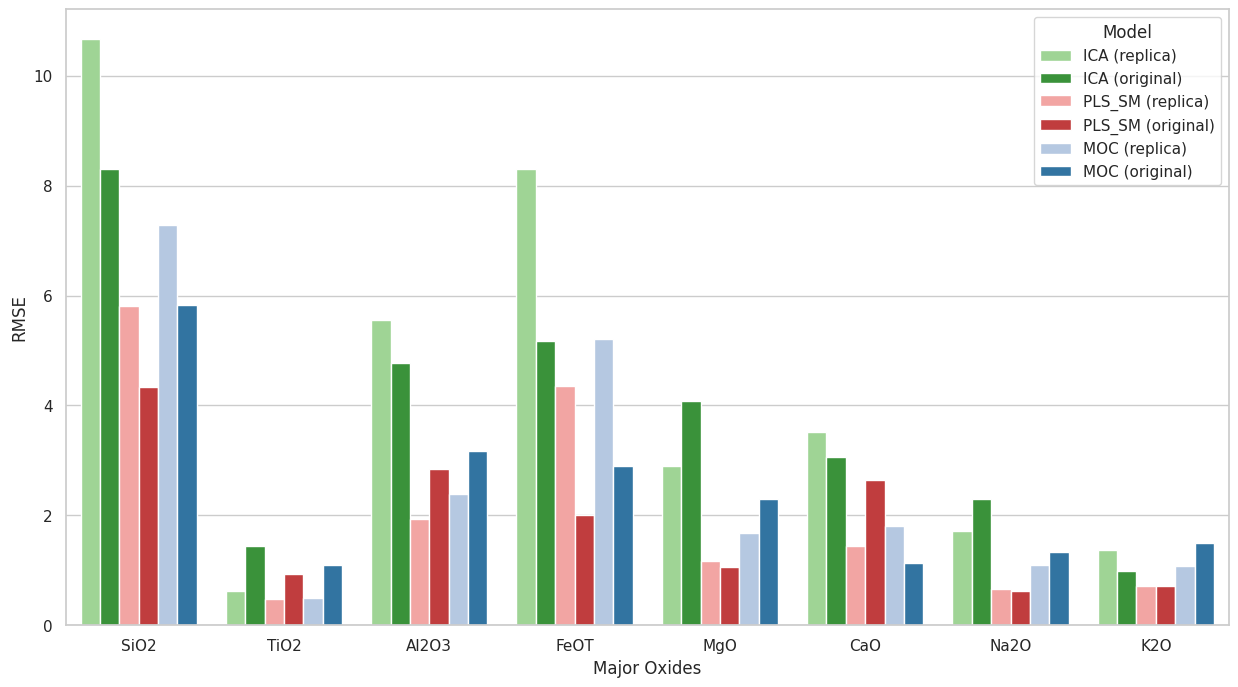
\includegraphics[width=0.85\textwidth]{images/rmse_historgram.png}
	\caption{Grouped histogram of the RMSEs of the original and our replicas of the PLS1-SM, ICA, and MOC models.}
	\label{fig:rmse_histograms}
\end{figure*}

\citet{andersonImprovedAccuracyQuantitative2017} used the Student's t-test to show their new model outperformed the old one. In our study, we apply the same test but with a different aim: to verify if there is no statistical significant difference between our replicated models (PLS1-SM, ICA, and MOC) and the original models presented in \citet{cleggRecalibrationMarsScience2017}. This approach allows us to assess whether our models demonstrate equivalence rather than improvement.
In conducting our analysis with the Student's t-test, we define our hypotheses and choose a significance level to guide our interpretation of the results.
Our null hypothesis (\(H_0\)) posits that there is no significant difference between the mean performance of our replicated models (PLS1-SM, ICA, and MOC) and that of the originals.
Conversely, the alternative hypothesis (\(H_1\)) suggests that there is a significant difference between the two sets of models.
We set a significance level (\(\alpha\)) of 5\%, which establishes the threshold for determining statistical significance.
If the p-value obtained from our t-test is less than 5\% (\(p < 0.05\)), we will reject the null hypothesis, indicating significant evidence of a difference between our replicated models and those of the original pipeline.
Conversely, if the p-value is greater than or equal to 5\% (\(p \geq 0.05\)), we fail to reject the null hypothesis, suggesting that our models and the original models are statistically similar, thereby achieving our goal of demonstrating equivalence rather than disparity.

Following the approach delineated in \citet{andersonImprovedAccuracyQuantitative2017}, we start by calculating the uncertainty of the RMSE values, $S_{RMSE}^2$:
$$
S_{\text{RMSE}}^2 = \left(\frac{\text{RMSE}^2}{n}\right) \left[n - 1 - \frac{2\Gamma^2\left(\frac{n}{2}\right)}{\Gamma^2\left(\frac{n - 1}{2}\right)}\right] \\
$$
where $n$ is the number of samples, and $\Gamma$ is the gamma function. This formulation captures the variance of the RMSE, reflecting the dispersion of error magnitudes.
Subsequently, the t-statistic $t$ is calculated to evaluate the statistical significance of the difference between the RMSEs of the original and replicated models:
$$
t = \frac{\text{RMSE}_A - \text{RMSE}_B}{\sqrt{S_{\text{RMSE}_A}^2 + S_{\text{RMSE}_B}^2}}
$$
where $\text{RMSE}_A$ and $\text{RMSE}_B$ correspond to the RMSE values of the original and replicated models, respectively.
The degrees of freedom ($f$) associated with this comparison are determined by:
$$
f = \frac{\left(S_{\text{RMSE}_A}^2 + S_{\text{RMSE}_B}^2\right)^2}{\frac{S^4_{\text{RMSE}_A}}{n_A - 1} + \frac{S^4_{\text{RMSE}_B}}{n_B - 1}}
$$
which accounts for the variances in RMSE values and the respective sample sizes ($n_A$ and $n_B$) of the models being compared.
Finally, the p-value is derived from the t-distribution's cumulative distribution function:
% Note to selves:
% This can be calculated using the cumulative distribution function of the t-distribution.
% https://stackoverflow.com/questions/17559897/python-p-value-from-t-statistic
% https://docs.scipy.org/doc/scipy/reference/generated/scipy.stats.t.html
% We've used: p_value = stats.t.sf(np.abs(t_value), degrees_of_freedom) * 2
% where t_value is the t-statistic and degrees_of_freedom is the degrees of freedom.
% But you could use: p_value = 2 * ( 1 - stats.t.cdf(abs(t_value), degrees_of_freedom))
% Just as well.
$$p\text{-value} = 2 \times \left(1 - F_{\text{T}}(|t|)\right)$$
where $F_{\text{T}}$ is the cumulative distribution function of the t-distribution with $f$ degrees of freedom.
Higher p-values indicate greater compatibility with the null hypothesis.

We present the results of our t-tests in Table~\ref{table:results_ttests}.

\begin{table}[h]
\centering
\begin{tabular}{llll}
\hline
Oxide & PLS1-SM & ICA & MOC \\
\hline
\ce{SiO2} & 42.00\% & 48.75\% & 38.45\% \\
\ce{TiO2} & 9.73\% & 6.31\% & 8.23\% \\
\ce{Al2O3} & 30.23\% & 67.06\% & 31.58\% \\
\ce{FeO_T} & 7.48\% & 21.68\% & 6.57\% \\
\ce{MgO} & 78.05\% & 35.44\% & 44.08\% \\
\ce{CaO} & 12.73\% & 70.04\% & 27.79\% \\
\ce{Na2O} & 85.96\% & 43.16\% & 14.93\% \\
\ce{K2O} & 100.00\% & 36.27\% & 43.40\% \\
\hline
\end{tabular}
\caption{Results of the PLS1-SM, ICA, and MOC t-tests}
\label{table:results_ttests}
\end{table}

The results from our t-tests are summarized as follows:

\begin{itemize}
    \item \textbf{PLS1-SM:} The p-values observed across the spectrum, most notably the 100.00\% for $K_2O$, unequivocally suggest a strong statistical proximity to the original models for a majority of the parameters. This is particularly indicative of a successful replication effort. However, the relatively lower p-value for $FeO_T$ (7.48\%) underscores an area where the model's performance diverges from the original. Given the high variance noted in the Section~\ref{sec:data_overview} for $FeO_T$ compositions, this deviation could be ascribed to inherent data variability rather than model inaccuracy.

    \item \textbf{ICA:} This model demonstrates considerable alignment with the original models across several constituents, as evidenced by p-values like 67.06\% for $Al_2O_3$ and 70.04\% for $CaO$. These figures indicate a noteworthy approximation to the original models' performance. Conversely, the p-value for $TiO_2$ (6.31\%) marks an exception, indicating a region where the ICA model might benefit from refinement. The noted high variance in $TiO_2$ values within our dataset likely contributes to this outlier, pointing to data variability as a contributing factor.

    \item \textbf{MOC:} The replicated MOC model's p-values, especially the 43.40\% for $K_2O$, reiterate its consistency with the original model's outcomes. This aligns with our hypothesis of statistical equivalence. Yet, as with PLS1-SM, the $FeO_T$ component exhibits a lower p-value (6.57\%), highlighting an area of divergence potentially attributed to the previously discussed variance in $FeO_T$ compositions.
\end{itemize}

This comparative analysis affirms a satisfying statistical equivalence between our replicated models and the original MOC models across most tested parameters.
This alignment underscores the robustness of our replication efforts.

However, the lower p-values associated with $FeO_T$ for both PLS1-SM and MOC, in addition to $TiO_2$ for ICA, flag these elements as focal points for potential refinement.
Given our dataset's inherent variability in the compositions of these specific elements, as substantiated in Section~\ref{sec:data_overview}, these findings are interpretable and not wholly unexpected.

In conclusion, our t-tests demonstrate that our replicated models are statistically similar to the original models, thereby achieving our goal of demonstrating equivalence rather than disparity.
As such, they serve their purpose as a baseline for identifying which aspects of the pipeline contribute the most to the overall error.

\begin{table*}[htbp] % Use htbp for more placement flexibility
\centering
\begin{tabular*}{\textwidth}{@{\extracolsep{\fill}} lllllll}
\hline
Model & RMSECV (avg) & RMSECV (min) & RMSEP & \# of spectra & \# Outliers removed & Outlier removal iterations  \\
\hline
SiO2 &&&&&& \\
  Low & 8.55 & 6.14 & 6.57 & 439 & 0 & 2 \\
  Mid & 4.71 & 3.64 & 4.20 & 1268 & 15 & 1 \\
  High & 3.59 & 3.01 & 4.26 & 605 & 1 & 2 \\
  Full & 5.98 & 4.75 & 7.18 & 1538 & 8 & 1 \\
\\
TiO2 &&&&&& \\
  Low & 0.29 & 0.28 & 0.39 & 1359 & 8 & 1 \\
  Mid & 0.62 & 0.57 & 0.44 & 418 & 6 & 4 \\
  High & 0.74 & 0.11 & 0.09 & 40 & 0 & 2 \\
  Full & 0.48 & 0.37 & 0.50 & 1538 & 16 & 4 \\
\\
Al2O3 &&&&&& \\
  Low & 2.40 & 1.68 & 1.99 & 324 & 0 & 2 \\
  Mid & 2.27 & 1.57 & 2.04 & 1198 & 12 & 2 \\
  High & 3.97 & 1.99 & 2.03 & 240 & 0 & 2 \\
  Full & 3.31 & 2.59 & 2.43 & 1538 & 9 & 1 \\
\\
FeOT &&&&&& \\
  Low & 1.81 & 1.72 & 1.55 & 1438 & 1 & 3 \\
  Mid & 2.64 & 2.15 & 1.69 & 978 & 28 & 9 \\
  High & 4.00 & 1.52 & 11.89 & 105 & 0 & 2 \\
  Full & 2.86 & 2.67 & 4.08 & 1538 & 23 & 5 \\
\\
MgO &&&&&& \\
  Low & 0.49 & 0.45 & 0.63 & 1000 & 7 & 4 \\
  Mid & 1.32 & 0.88 & 1.16 & 1488 & 10 & 1 \\
  High & 4.42 & 1.99 & 3.14 & 135 & 0 & 1 \\
  Full & 1.74 & 1.36 & 1.25 & 1538 & 41 & 6 \\
\\
CaO &&&&&& \\
  Low & 0.79 & 0.57 & 0.78 & 1070 & 22 & 6 \\
  Mid & 1.40 & 1.07 & 1.02 & 1428 & 20 & 4 \\
  High & 1.89 & 0.72 & 1.85 & 35 & 0 & 2 \\
  Full & 1.62 & 1.19 & 1.81 & 1538 & 41 & 8 \\
\\
Na2O &&&&&& \\
  Low & 0.57 & 0.48 & 0.57 & 1278 & 8 & 3 \\
  High & 1.27 & 0.65 & 0.60 & 375 & 0 & 1 \\
  Full & 1.05 & 0.59 & 1.00 & 1538 & 37 & 7 \\
\\
K2O &&&&&& \\
  Low & 0.39 & 0.28 & 0.34 & 773 & 5 & 3 \\
  High & 0.98 & 0.58 & 0.71 & 920 & 13 & 2 \\
  Full & 1.03 & 0.92 & 0.81 & 1538 & 48 & 8 \\
\\

\end{tabular*}
\caption{Summary of PLS model performance for the major oxides.}
\label{table:rmsecv_results}
\end{table*}


\subsection{Experiment: PLS Automated Outlier Removal}\label{sec:experiment_pls_automated_outlier_removal}
When \citet{cleggRecalibrationMarsScience2017} developed the PLS1-SM models, outliers were removed based on manual inspection of the leverage and spectral residuals plots.
We have instead chosen to automate this based on the reasons described in Section~\ref{sec:methodology_outlier_removal}.
As such, examining the performance implications of completely omitting outlier removal would be worthwhile.
This experiment is justified given the substantial efforts dedicated to developing the ChemCam calibration dataset as mentioned in Section~\ref{sec:ica_data_preprocessing}, which implies a minimal presence of significant outliers.

Table \ref{tab:pls1_sm_no_outlier_rmses} shows the RMSEs for the PLS1-SM replica model with and without automated outlier removal.
The RMSEs are very similar, which indicates that the automated outlier removal does not have a significant impact on the model performance.
This is expected based on the aforementioned efforts that went into developing the ChemCam calibration dataset, as described in Section~\ref{sec:ica_data_preprocessing}.

\begin{table}[h]
\centering
\begin{tabular}{lll}
\hline
Element    & Baseline & Without outlier removal \\
\hline
\ce{SiO2}  & 5.81     & 5.81                    \\
\ce{TiO2}  & 0.47     & 0.47                    \\
\ce{Al2O3} & 1.94     & 1.91                    \\
\ce{FeO_T} & 4.35     & 4.35                    \\
\ce{MgO}   & 1.17     & 1.17                    \\
\ce{CaO}   & 1.43     & 1.44                    \\
\ce{Na2O}  & 0.66     & 0.67                    \\
\ce{K2O}   & 0.72     & 0.70                    \\
\hline
\end{tabular}
\caption{RMSEs for the PLS1-SM model without automated outlier removal.}
\label{tab:pls1_sm_no_outlier_rmses}
\end{table}


% TODO: Results and discussion here.

\subsection{Experiment: PLS Fixed Thresholds}\label{sec:experiment_pls_fixed_thresholds}
We maintained the leverage and residuals from the second iteration of the outlier removal in the PLS1-SM training process, leading to a more conservative outlier removal process where fewer samples are removed.
The reason for doing so was that we did not know the basis for the original author's manual outlier removal process, and it is possible that they were more conservative than our automated process.
Consequently, a more conservative approach could potentially align our replica of the pipeline more closely with the original.

Table \ref{tab:pls1_sm_fixed_thresholds_rmses} shows the RMSEs for the PLS1-SM baseline model with fixed outlier removal thresholds.
The RMSEs are almost identical, which further reinforces the conclusion from the previous experiment that the automated outlier removal does not have a significant impact on the model performance.

\begin{table}[h]
\centering
\begin{tabular}{lll}
\hline
Element    & Baseline      & Fixed thresholds \\
\hline
\ce{SiO2}  & \textbf{5.81}          & \textbf{5.81}  \\
\ce{TiO2}  & \textbf{0.47}          & \textbf{0.47}  \\
\ce{Al2O3} & \textbf{1.94}          & \textbf{1.94}  \\
\ce{FeO_T} & \textbf{4.35}          & \textbf{4.35}  \\
\ce{MgO}   & \textbf{1.17}          & 1.18           \\
\ce{CaO}   & \textbf{1.43}          & 1.44           \\
\ce{Na2O}  & \textbf{0.66}          & 0.6            \\
\ce{K2O}   & \textbf{0.72}          & \textbf{0.72}  \\
\hline
\end{tabular}
\caption{RMSEs for the PLS1-SM model with fixed outlier removal thresholds.}
\label{tab:pls1_sm_fixed_thresholds_rmses}
\end{table}

\subsection{Experiment: ICA MAD Outlier Removal}\label{sec:experiment_ica_mad_outlier_removal}
In the ICA phase, the original authors employed the Median Absolute Deviation (MAD) for outlier removal, yet the detailed methodology of their approach was not fully delineated.
Consequently, in our version of the pipeline, we chose to exclude the outlier removal step during the ICA phase to avoid introducing unsubstantiated assumptions, as described in Section~\ref{sec:ica_data_preprocessing}.
This decision allowed us to evaluate the intrinsic effectiveness of the ICA phase without outlier removal and assesses the impact of introducing MAD (Median Absolute Deviation) for outlier removal in our pipeline replication.
By comparing results with and without MAD, we aim to quantitatively determine its utility in reducing noise and improving data quality.
This will also provide insights into the robustness of the ICA phase against outliers, offering a comprehensive understanding of the pipeline's capabilities and limitations.

As mentioned in Section~\ref{sec:ica_data_preprocessing}, \citet{cleggRecalibrationMarsScience2017} did not specify the exact methodology of their outlier removal process.
Therefore, we experimented with applying it at different stages of the ICA phase.
The results presented in Table~\ref{tab:ica_mad_rmses} are the best results we obtained from these experiments, which were achieved by applying MAD before masking and normalization in the preprocessing phase.

\begin{table}[h]
\centering
\begin{tabular}{lll}
\hline
Element    & ICA baseline   & ICA with MAD \\
\hline
\ce{SiO2}  & 10.68          & \textbf{8.64} \\
\ce{TiO2}  & 0.63           & \textbf{0.53} \\
\ce{Al2O3} & 5.55           & \textbf{3.69} \\
\ce{FeO_T} & 8.30           & \textbf{7.07} \\
\ce{MgO}   & 2.90           & \textbf{2.10} \\
\ce{CaO}   & \textbf{3.52}  & 4.00 \\
\ce{Na2O}  & 1.72           & \textbf{1.45} \\
\ce{K2O}   & 1.37           & \textbf{1.15} \\
\hline
\end{tabular}
\caption{RMSEs for the ICA phase's regression models with and without MAD-based outlier removal.}
\label{tab:ica_mad_rmses}
\end{table}

As evident from Table~\ref{tab:ica_mad_rmses}, the ICA phase's performance is improved across all elements when MAD is applied except for $\ce{CaO}$.
We hypothesize that this could be because the nature of the $\ce{CaO}$ data might differ from other elements, where outliers removed according to the MAD-based approach might be removing critical information, resulting in a less accurate model.

It is also notable that the ICA regression models show an overall significant improvement when outlier removal is applied, while the experiment presented in Section~\ref{sec:experiment_pls_automated_outlier_removal} shows that omitting outlier removal in the PLS1-SM phase does not have a significant impact on the models' performance.
This indicates that PLS is more robust to outliers than ICA.

Given these results, we decided to recalculate the MOC $t$-test results given the RMSEs from the ICA phase with MAD-based outlier removal.
The results, along with the previous $t$-test values for comparison, are presented in Table~\ref{tab:ica_mad_moc_ttest_results}.
\begin{table}[h]
\centering
\begin{tabular}{lllll}
\hline
Element & \multicolumn{2}{c}{ICA} & \multicolumn{2}{c}{MOC} \\
& Replica & MAD & Replica & MAD \\
\hline
\ce{SiO2} & 48.75\% & 91.22\% & 38.45\% & 56.64\% \\
\ce{TiO2} & 6.31\% & 3.91\% & 8.23\% & 5.87\% \\
\ce{Al2O3} & 67.06\% & 47.80\% & 31.58\% & 18.10\% \\
\ce{FeOT} & 21.68\% & 39.26\% & 6.57\% & 7.83\% \\
\ce{MgO} & 35.44\% & 10.76\% & 44.08\% & 15.57\% \\
\ce{CaO} & 70.04\% & 46.52\% & 27.79\% & 49.03\% \\
\ce{Na2O} & 43.16\% & 23.06\% & 14.93\% & 30.33\% \\
\ce{K2O} & 36.27\% & 65.36\% & 43.40\% & 63.77\% \\
\hline
\end{tabular}
\caption{Comparison of element percentages in ICA and MOC methods with replica and MAD-based approaches.}
\label{tab:ica_mad_moc_ttest_results}
\end{table}

As shown in Table~\ref{tab:ica_mad_moc_ttest_results}, using MAD-based outlier removal in the ICA phase results in a significant improvement in the MOC $t$-test results for all elements except \ce{SiO2}, \ce{TiO2}, and \ce{CaO}. 
This indicates that MAD-based outlier removal is effective in improving the ICA phase's performance.
It also suggests that the ICA phase is more susceptible to outliers than the PLS1-SM phase, as the PLS1-SM phase's performance was not significantly impacted by the omission of outlier removal.
We will examine this further in the next experiment in Section~\ref{sec:experiment_ica_aggregated_datasets}.

In Section~\ref{sec:ica_data_preprocessing}, we explained why we did not use the inverse of the IRF for weighting, based on critique from one of the original authors of \citet{cleggRecalibrationMarsScience2017}.
Based on the fact that our ICA replica, which does not utilize the inverse of the IRF for weighting, yields results similar to the original ICA method, we concur with the original author's critique that weighting by the inverse of the IRF lacks justification.

\subsection{Experiment: ICA Aggregated Datasets}\label{sec:experiment_ica_aggregated_datasets}
In Section~\ref{sec:ica_data_preprocessing}, we described how we only use one of the five location datasets for each sample for the ICA training process.
In this experiment, we used all five location datasets for each sample, and aggregated the results by taking the mean of the shots over the datasets.
Since this results in an averaged dataset, we expect to either lose information by averaging out the differences between the datasets, or gain information by reducing the noise in the dataset.

Table \ref{tab:ica_aggregated_rmses} shows the RMSEs for the ICA model with and without aggregated datasets.

\begin{table}[h]
\centering
\begin{tabular}{lll}
\hline
Element    & Baseline      & Aggregated datasets \\
\hline
\ce{SiO2}  & 5.81          & 12.01 \\
\ce{TiO2}  & 0.47          & 0.60 \\
\ce{Al2O3} & 1.94          & 4.81 \\
\ce{FeO_T} & 4.35          & 8.56 \\
\ce{MgO}   & 1.17          & 2.51 \\
\ce{CaO}   & 1.43          & 3.71 \\
\ce{Na2O}  & 0.66          & 1.41 \\
\ce{K2O}   & 0.72          & 1.51 \\
\hline
\end{tabular}
\caption{RMSEs for the ICA phase's regression models using aggregated datasets.}
\label{tab:ica_aggregated_rmses}
\end{table}

The results, as depicted in Table~\ref{tab:ica_aggregated_rmses}, indicate a significant increase in the Root Mean Square Error (RMSE) across all elements when aggregated datasets were used compared to the baseline.
Specifically, the RMSE values for \ce{SiO2}, \ce{Al2O3}, \ce{FeO_T}, \ce{MgO}, \ce{CaO}, \ce{Na2O}, and \ce{K2O} all saw substantial increases.
This suggests that the aggregation process, contrary to potentially enhancing model accuracy by noise reduction, actually led to a considerable loss of critical information necessary for accurate predictions.

Such an outcome implies that the variability between the different location datasets contains valuable information that is pertinent to the predictive modeling of oxide compositions.
Averaging these datasets seems to dilute these nuances, leading to a generalized representation of the samples that does not capture the specificities required for precise predictions.
This is particularly evident in the case of \ce{SiO2} and \ce{Al2O3}, where the RMSE more than doubled when using aggregated datasets, highlighting a significant degradation in model performance.

\subsection{Experiment: Other Models}\label{sec:experiment_other_models}
\citet{cleggRecalibrationMarsScience2017} have only compared their new approach with the original method presented by \citet{wiensPreFlight3}, and have not conducted experiments using alternative methods to establish the superiority of their chosen approach.
Therefore, we decided to compare the performance of the PLS1-SM and ICA models to other models.
The objective was to evaluate two distinct scenarios.
In the first scenario, we aimed to conduct a direct comparison between the MOC model and an alternative model. The second scenario revolves around substituting either PLS or ICA with a different model and then calculating a weighted average.
We have decided to conduct the experiments using the following models:

\begin{itemize}
	\item \textbf{XGBoost}, a gradient boosting algorithm \cite{chen_xgboost_2016}
	\item \textbf{ANN}, a neural network model
\end{itemize}

Building on the findings of \citet{andersonPostlandingMajorElement2022}, who demonstrated Gradient Boosting Regression (GBR) models' superior predictive accuracy in analyzing major oxide compositions in geological samples, we adopt XGBoost for its refined GBR implementation.
This decision is informed by XGBoost's documented success in enhancing model precision, as detailed in Section~\ref{sec:related_works}.

In light of \citeauthor{takahashi_quantitative_2017}'s findings on the limitations of traditional LIBS calibration methods and the potential of ANNs to address non-linearities in solid sample analysis, described in Section~\ref{sec:related_works}, we also decided to include ANNs in our experiments.
This approach is motivated by ANNs' capacity to discern complex, non-linear relationships within LIBS spectra.

The ANN comprises of a sequence of fully connected (dense) layers and dropout layers, aimed at reducing overfitting through regularization.
The architecture begins with an input layer of 6144 units, reflecting the high-dimensional nature of the input data.
This is immediately followed by a series of linear transformations and non-linear activations (ReLU), reducing the dimensionality in a stepwise fashion to 1024, 512, 256, and finally 128 units across four layers.
Each of these reductions is aimed at distilling the essential features required for accurate regression outcomes.
The inclusion of dropout layers with a dropout rate of 0.3 after the first and second dense layers further aids in mitigating the risk of overfitting by randomly omitting a subset of features during the training phase.
The final layer of ANN outputs 8 variables, corresponding to the eight major oxides we are trying to predict the compositional values of.
Notably, this layer does not employ an activation function, as it aims to produce linear outputs that directly correspond to the predicted values for each of the regression targets.


\begin{table*}[h]
\centering
\begin{tabular}{lllllll}
\hline
Element    & ANN (Norm1)   & ANN (Norm3) & XGBoost (Norm1) & XGBoost (Norm3) & MOC (original) & MOC (replica) \\
\hline
\ce{SiO2}  & 5.62          & 5.01        & 5.12            & \textbf{4.67}   & 5.30           & 7.29 \\
\ce{TiO2}  & 0.58          & 0.62        & \textbf{0.44}   & 0.45            & 1.03           & 0.49 \\
\ce{Al2O3} & 2.12          & 2.27        & \textbf{1.93}   & 1.97            & 3.47           & 2.39 \\
\ce{FeO_T} & 4.05          & 4.00        & 4.40            & 5.02            & \textbf{2.31}  & 5.21 \\
\ce{MgO}   & 1.61          & 1.49        & 0.99            & \textbf{0.96}   & 2.21           & 1.67 \\
\ce{CaO}   & 1.33          & 1.26        & \textbf{1.23}   & 1.26            & 2.72           & 1.81 \\
\ce{Na2O}  & 1.17          & 1.09        & \textbf{0.49}   & 0.51            & 0.62           & 1.10 \\
\ce{K2O}   & 1.05          & 0.88        & \textbf{0.50}   & 0.51            & 0.82           & 1.09 \\
\hline
\end{tabular}
\caption{RMSEs for the ANN and XGBoost models using Norm 1 and Norm 3. The RMSEs for the MOC models are included for comparison.}
\label{tab:other_models_rmses}
\end{table*}

The results presented in Table~\ref{tab:other_models_rmses} provide a comparison of the RMSE metric performance between the artificial neural network (ANN), XGBoost models, and the MOC (Model of Calibration) under two normalization conditions (Norm 1 and Norm 3), across the eight major oxides.

Overall, the results suggest that XGBoost, particularly under the Norm 1 condition, consistently provides superior predictive accuracy for most of the oxides analyzed, with the exception of \ce{FeO_T} where the original MOC model excels.
This indicates the potential benefits of integrating advanced machine learning techniques, such as gradient boosting, into the analysis of LIBS data for geological samples.
The superior performance of XGBoost could be attributed to its sophisticated handling of complex data structures and its ability to minimize overfitting, making it a robust choice for predictive modeling in this context.

ANNs also show promising results, particularly in scenarios where traditional models might not capture complex non-linear relationships effectively.
However, their performance is generally outperformed by XGBoost, suggesting that while ANNs have the capacity to model complex phenomena within LIBS spectra, the specific architecture and training procedures might need further optimization to fully leverage their potential.
The relatively small training dataset might also be a contributing factor to the ANN's performance, as ANNs typically require a large amount of data to train effectively.


\subsection{summary}\label{sec:experiments_summary}
The experiments conducted in this section provide an assessment of the MOC pipeline's components, offering insights into their individual and collective impacts on the system's overall performance.

Our findings indicate that outlier removal does not have a major impact on neither the PLS1-SM nor the ICA models, which is expected considering we anticipate a low number of outliers in the dataset, as mentioned in Section~\ref{ica_data_preprocessing}.
Following this, we also found that maintaining the leverage and residuals from the second iteration of the outlier removal barely affects the PLS1-SM model's performance.

We also found that the MAD method for outlier removal in the ICA phase improves the performance of the ICA models across all oxides except for \ce{CaO}.
When using all five datasets for training the ICA models through aggregation, we found that the RMSEs vary across the oxides, with oxides that have a higher variance in their compositions having higher RMSEs and vice versa.

Finally, we found that the XGBoost model performs exceptionally well, only being outperformed by the original MOC model on \ce{FeO_T}.
The ANN model also shows promising results, often outperforming the original MOC model, and we expect that it could perform even better with a larger training dataset.

We can draw several key conclusions from the experiments conducted in this section regarding the limitations of the MOC pipeline components:

% TODO: Key conclusion here - what is the key limitations of the MOC pipeline components?
% Note that PLS was more robust to outliers than ICA! The RMSEs for ICA were much higher than PLS when we did not do outlier removal.

Finally, an aspect that is out of scope for this study is the inherent limitations stemming from the calibration dataset itself.
The fact that it was acquired on Earth and not on Mars, and that it was acquired using a different LIBS instrument than the one used on Mars, causes a misalignment between the calibration dataset and the unseen data gathered by Mars rovers.
In fact, NASA acknowledges this limitation, and is currently working on a mission to bring samples from Mars back to Earth, where they can be analyzed in laboratories around the world \cite{mars-sample-return}.
This would allow for the creation of a calibration dataset that is more representative of the unseen data, which would allow for more accurate predictions.
